\section{Specifications}
\label{sec:specs}
\newcounter{SpecID}

\subsection{Arena}
\refstepcounter{SpecID}
\label{spec:arena}

\begin{enumerate}
  \item The arena floor is an \SI{9}{m} $\times$ \SI{9}{m} rectangle. The
        tolerance of these two dimensions is $\pm$ \SI{250}{mm}.
  \item The floor of the arena is carpeted.
  \item The layout of the arena is given in Figure~\ref{fig:arena}. This
        figure is to scale.
  \item The outer walls of the arena are at least \SI{600}{mm} high, and the
        interior surface is white plastic-coated hardboard.
  \item The raised area is \SI{2.4}{m} $\times$ \SI{2.4}{m} $\pm$ \SI{100}{mm},
        with a height of \SI{180}{mm} $\pm$ \SI{10}{mm}.
  \item The scoring zones extend a further \SI{2.4}{m} $\times$ \SI{2.4}{m} $\pm$ \SI{100}{mm}
        from the raised area, resulting in a total size of \SI{4.8}{m} $\times$ \SI{4.8}{m} $\pm$ \SI{200}{mm}.
  \item Scoring zones will be bounded by metallic tape around the perimeter
        and internal boundaries. The inside edge of the tape marks the outside
        edge of the scoring zone.
  \item At the cardinal points of the arena are \SI{1.2}{m} $\times$ \SI{1.2}{m} $\pm$ \SI{100}{mm} walls,
        raised at least \SI{180}{mm} $\pm$ \SI{10}{mm}.
  \item Scoring zones for teams will be offset 90\degree{} anti-clockwise, such
        that a team isn't directly in front of their own scoring zone.
  \item Each robot will be assigned a corner at the start of every match to indicate its starting area.
        Corner starting areas are \SI{1000}{mm} $\pm$ \SI{20}{mm} square and will be marked by tape.
\end{enumerate}

\begin{figure}
  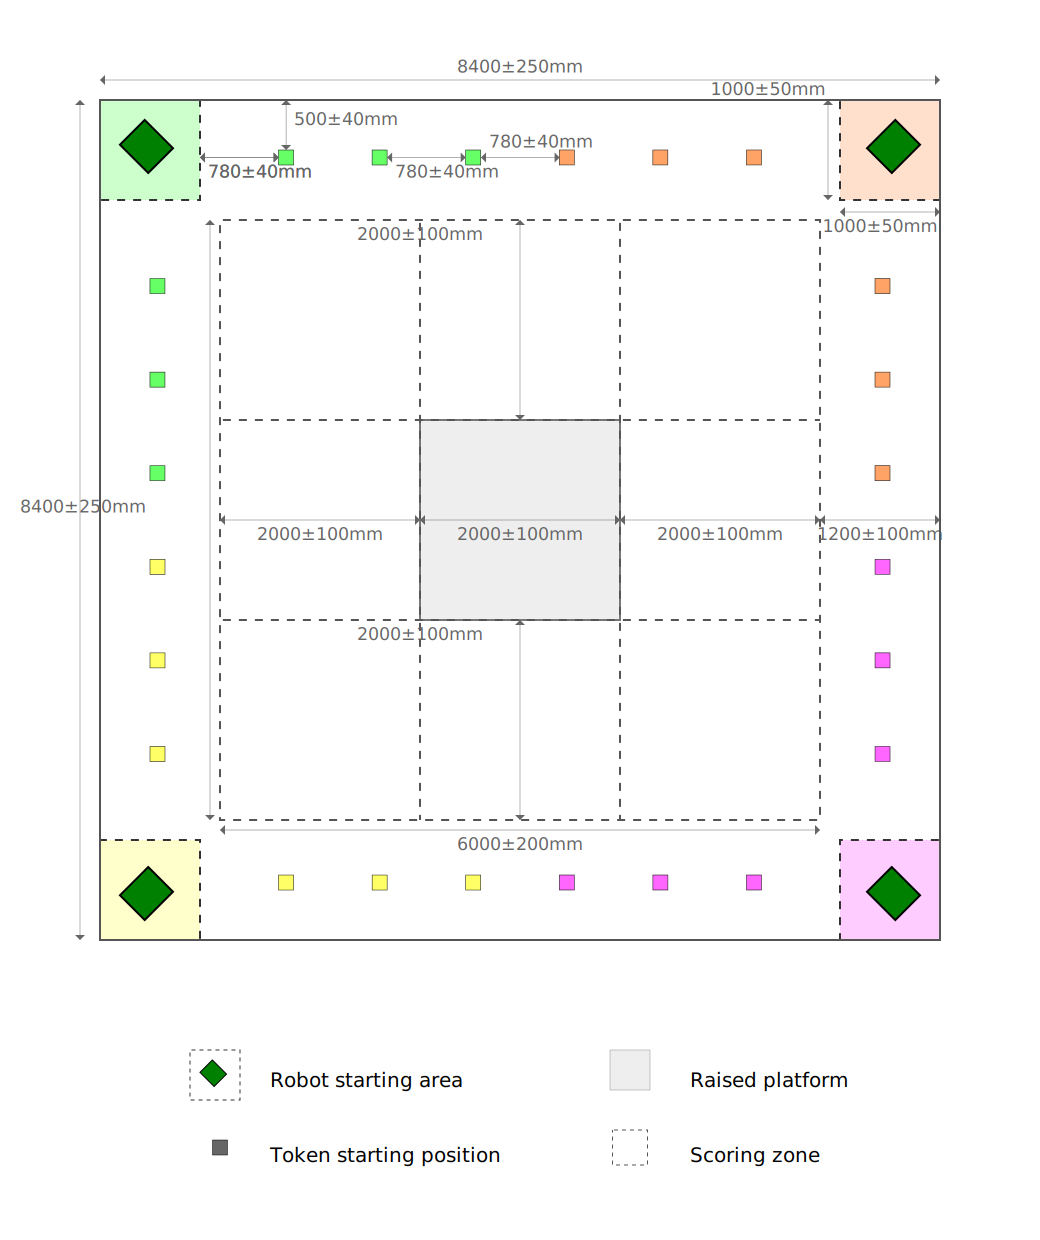
\includegraphics[scale=0.58]{fig-arena.pdf}
  \caption{Layout zones and tokens in the arena.}
  \label{fig:arena}
\end{figure}

\subsection{Tokens}
\refstepcounter{SpecID}
\label{spec:tokens}

\begin{enumerate}
  \item The tokens are cuboids with side length \SI{250}{mm} $\pm$ \SI{10}{mm}.
  \item Each face of each token is bordered by \SI{10}{mm} $\pm$ \SI{2}{mm} of
        copper conductive tape.
  \item There are 20 possible starting positions for tokens in the arena. These
        are arranged as indicated in Figure~\ref{fig:arena}.
  \item At the start of each match each quadrant four of the starting positions
        in each quadrant will be occupied. The position nearest the starting
        area of each quadrant will always be occupied.
  \item While the token starting positions are rotationally symmetrical, the
        pattern of which are occupied in any given match may not be.
\end{enumerate}
